\newpage
\section{Resultados}

\subsection{Calculo do indutor}

Para o calculo do indutor, foi criado o \textit{script} do MATLAB mostrado abaixo:


clear all 
close all
clc

syms L1 
w0 = 2 * pi * 4e6;
C1 = 470e-12;
C2 = 10e-9;
 
eq = w0 == 1 / (sqrt(L1*((C1*C2)/(C1+C2))));

L = double(solve(eq,L1))


\subsection{Citcuito 2}

Para o primeiro estágio, a frequência de corte teórica é $f_{c1} = 4545 \quad [Hz]$ e a frequência de corte simulada é $f_{c1} = 4398 \quad [Hz]$. A figura \ref{f_bode2} mostra o gráfico da resposta em frequência do primeiro estágio. Este filtro é um Chebyshev passa-baixas, com atenuação -38,7 dB/década (segunda ordem) e ganho de -151 [V/V].
Note que o valor do ganho é negativo devido ao amplificador inversor.

\begin{figure}[H]
\centering
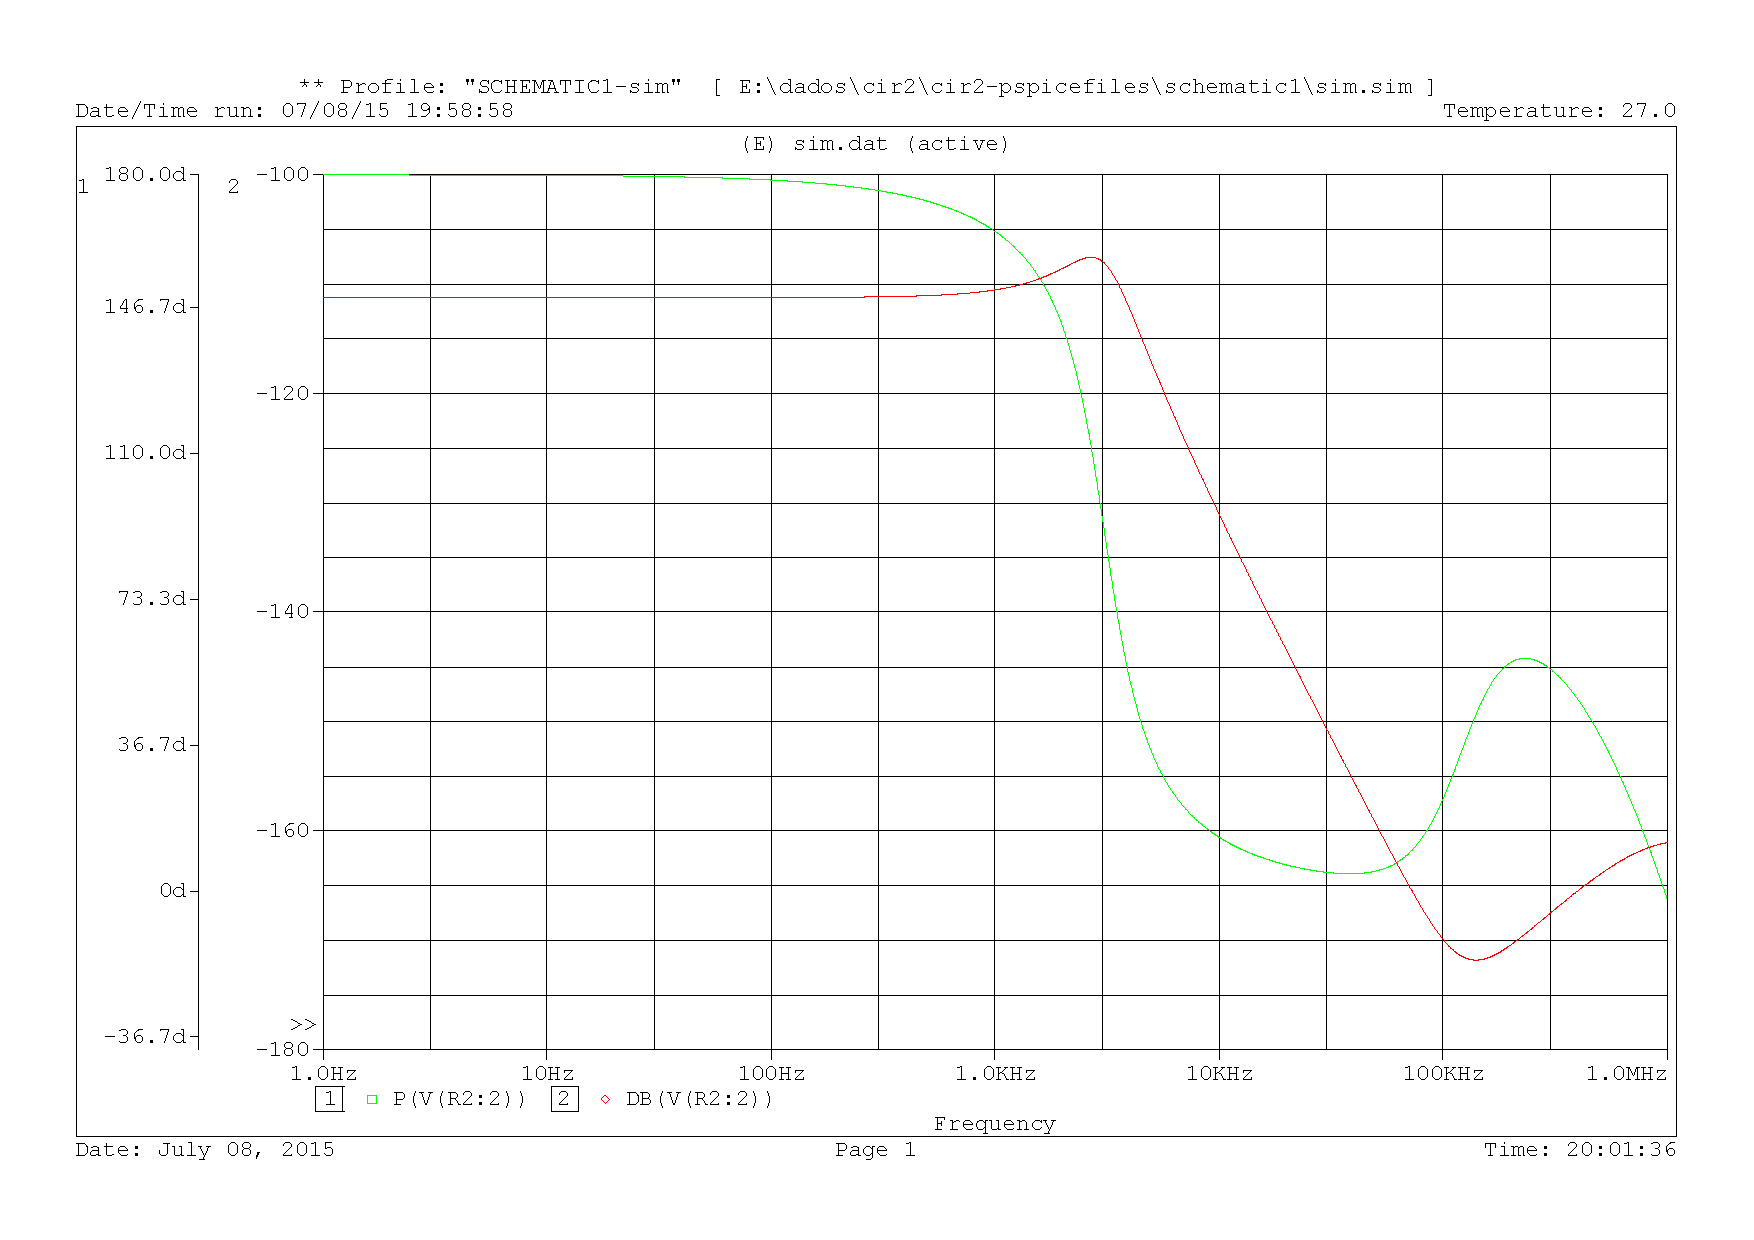
\includegraphics[scale=0.5]{Imagens/bode2.pdf}
\caption{Frequência e fase para primeiro estágio do filtro em cascata.}
\label{f_bode2}
\end{figure}


Para o segundo estágio, a frequência de corte teórica é $f_{c1} = 3150 \quad [Hz]$ e a frequência de corte simulada é $f_{c1} = 3039 \quad [Hz]$. A figura \ref{f_bode3} mostra o gráfico da resposta em frequência do segundo estágio. Este filtro é um passa-baixas, com atenuação -40 dB/década (segunda ordem) e ganho de -154 [V/V].
Note que o valor do ganho é negativo devido ao amplificador inversor.

\begin{figure}[H]
\centering
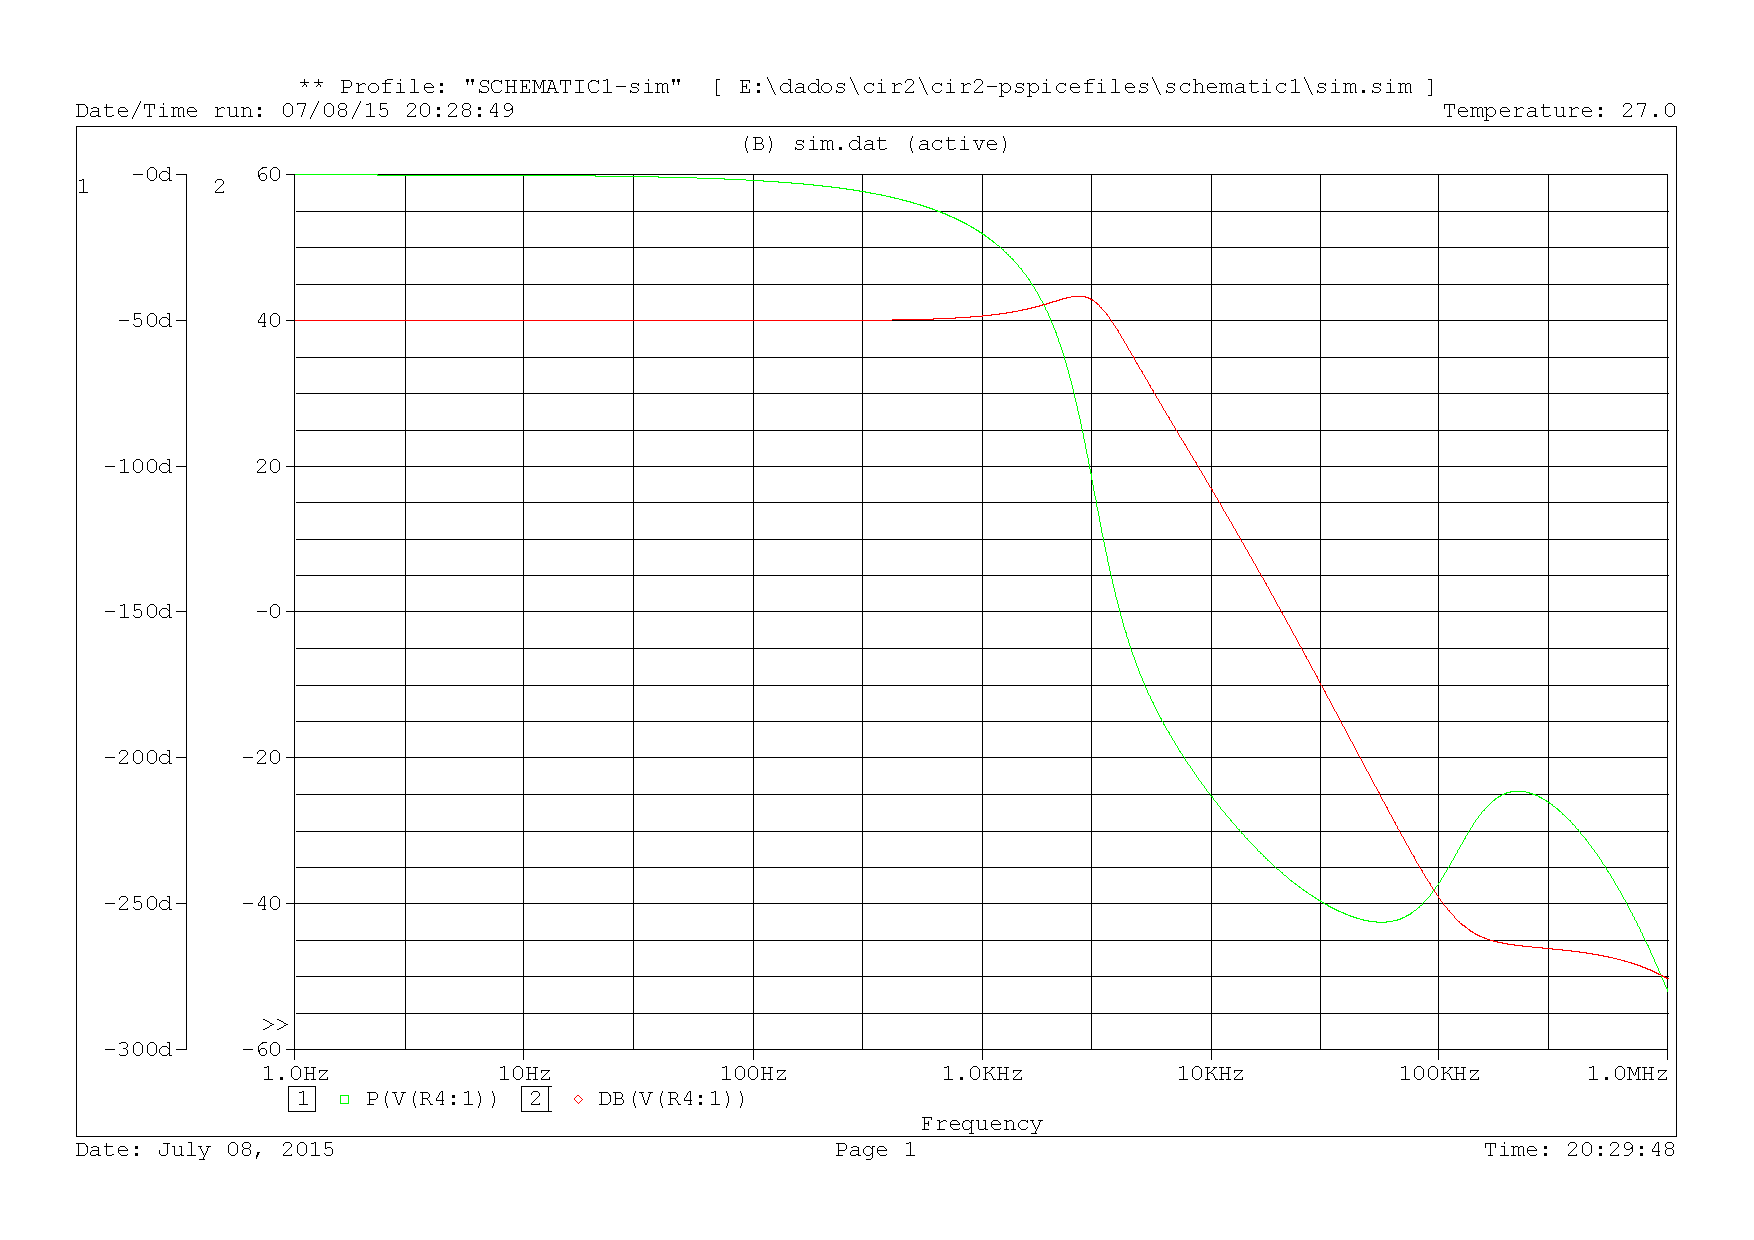
\includegraphics[scale=0.5]{Imagens/bode3.pdf}
\caption{Frequência e fase para segundo estágio do filtro em cascata.}
\label{f_bode3}
\end{figure}

A saída do amplificador em cascata é exibida na figura \ref{f_bode4}, onde foi encontrado que a frequência de corte é de $f_{c1} = 2735 \quad [Hz]$. O filtro possui resposta em frequência do tipo passa baixas de ordem quatro, com atenuação de -22dB/oitava.

\begin{figure}[H]
\centering
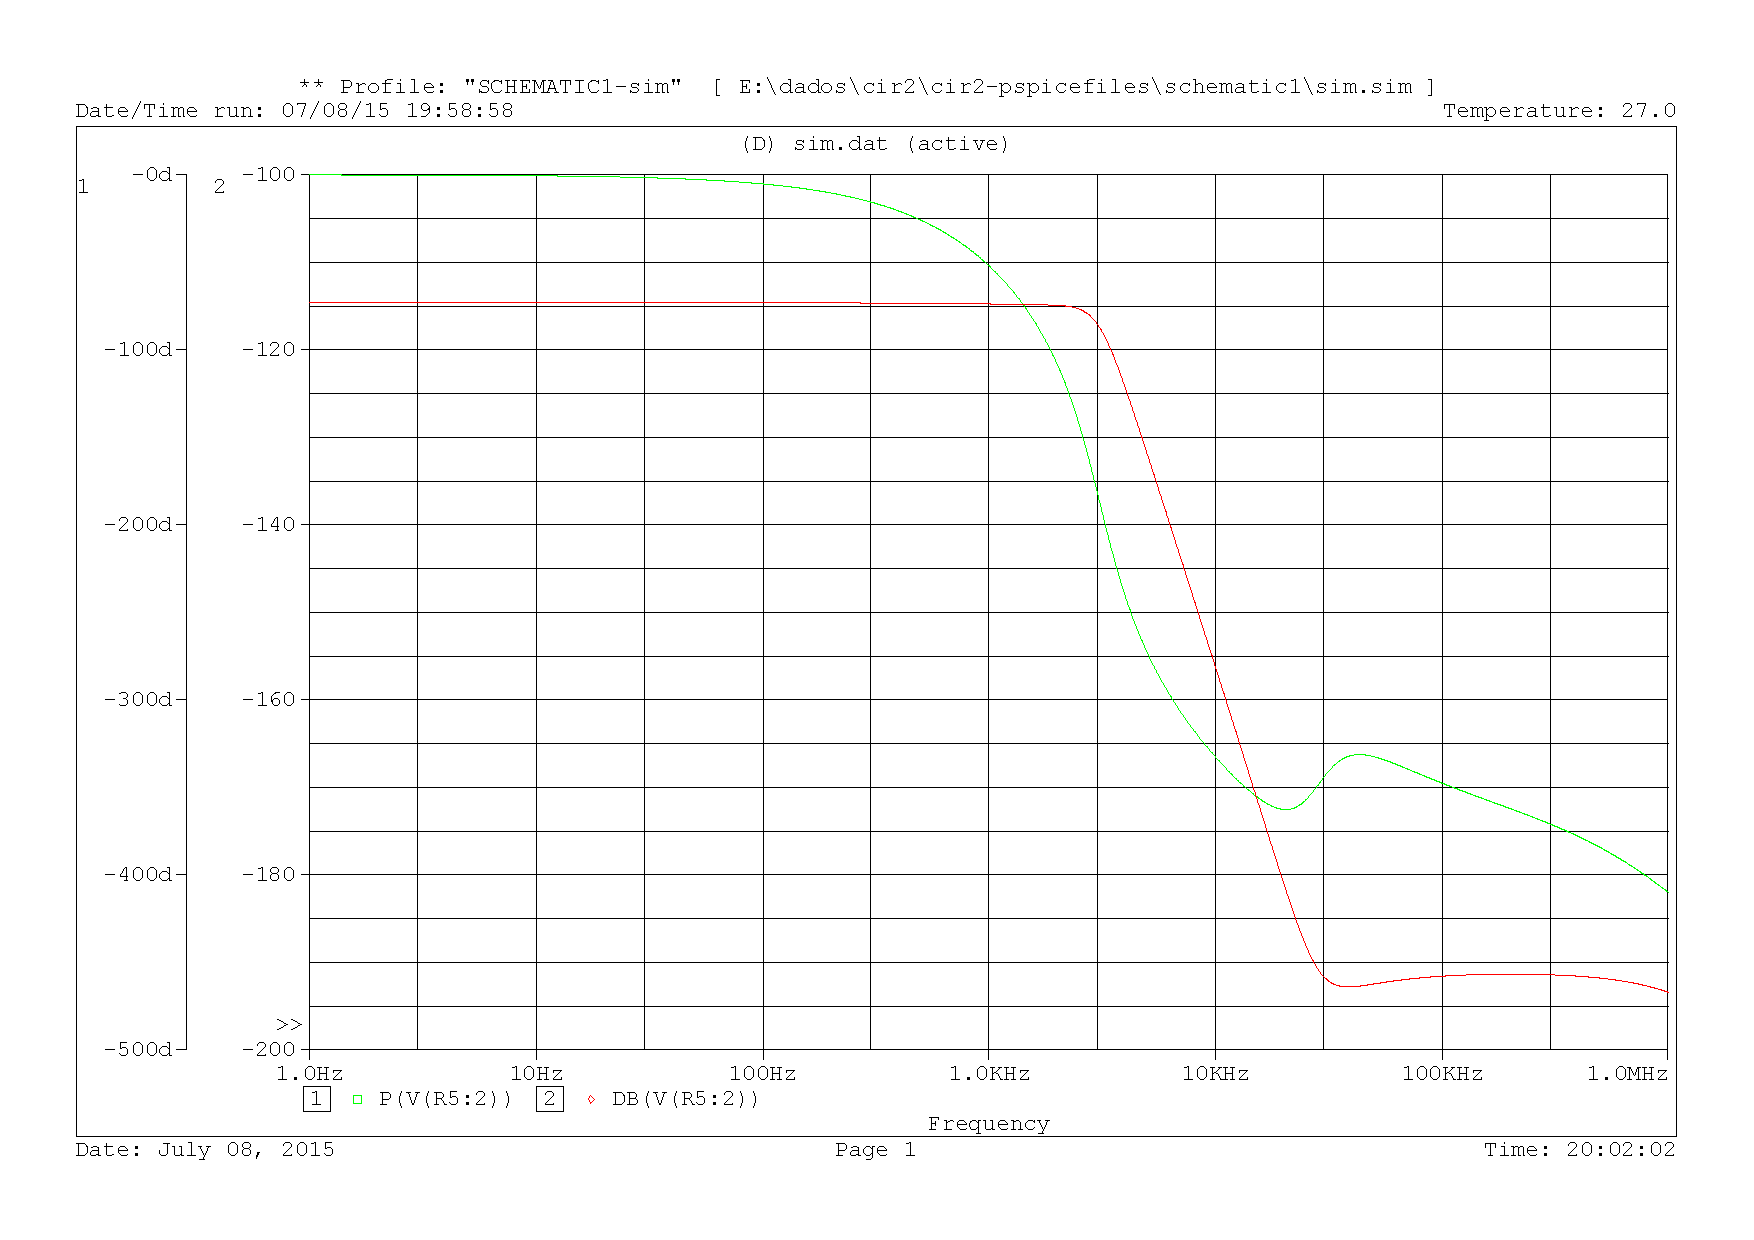
\includegraphics[scale=0.5]{Imagens/bode4.pdf}
\caption{Frequência e fase para primeiro estágio do filtro em cascata.}
\label{f_bode4}
\end{figure}

Para a ultima etapa, foi inserido um sinal de onda quadrada com frequência de 2461 Hz na entrada do filtro em cascata. A onda encontrada na saída está na figura \ref{f_square}.

\begin{figure}[H]
\centering
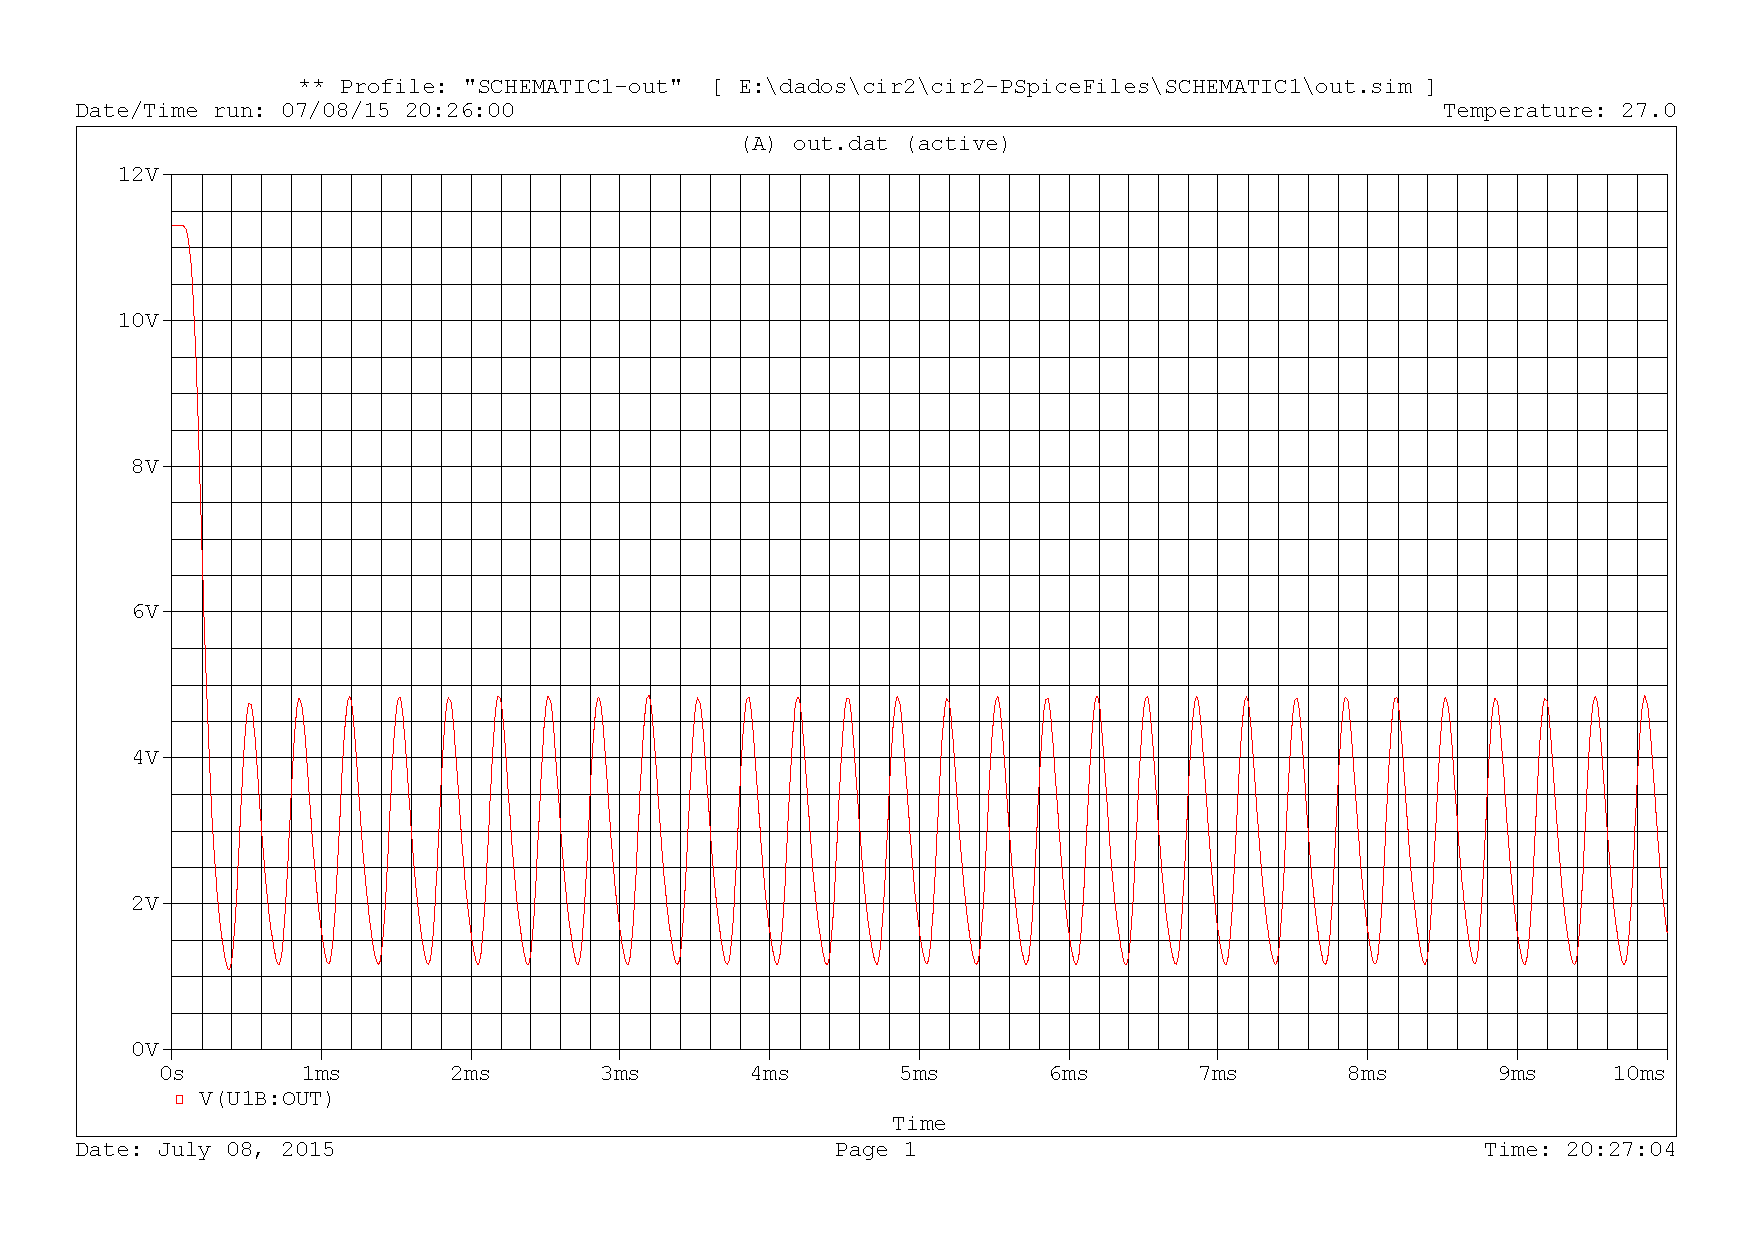
\includegraphics[scale=0.5]{Imagens/square.pdf}
\caption{Frequência e fase para primeiro estágio do filtro em cascata.}
\label{f_square}
\end{figure}
